%%%%%%%%%%%%%%%%%%%%%%%%%%%%%%%%%%%%%%%%%%%%%%%%%%%%%%%%%%%%
%%  Class 1, NE 155
%%

\documentclass[xcolor=x11names,compress]{beamer}

\definecolor{CoolBlack}{rgb}{0.0, 0.18, 0.39}
%% General document %%%%%%%%%%%%%%%%%%%%%%%%%%%%%%%%%%
\usepackage{graphicx}
\usepackage{tikz}
\usetikzlibrary{decorations.fractals}
\usepackage{hyperref}
%%%%%%%%%%%%%%%%%%%%%%%%%%%%%%%%%%%%%%%%%%%%%%%%%%%%%%

%% Beamer Layout %%%%%%%%%%%%%%%%%%%%%%%%%%%%%%%%%%
\useoutertheme[subsection=false,shadow]{miniframes}
\useinnertheme{default}
\usefonttheme{serif}
\usepackage{palatino}
\usepackage{tabu}
% Links
\usepackage{hyperref}
\definecolor{links}{HTML}{003262}
\hypersetup{colorlinks,linkcolor=,urlcolor=links}

% addition of color
\usepackage{xcolor}
\definecolor{CoolBlack}{rgb}{0.0, 0.18, 0.39}
\definecolor{byellow}{rgb}{0.55037, 0.38821, 0.06142}
\definecolor{dgreen}{rgb}{0.,0.6,0.}
\definecolor{RawSienna}{cmyk}{0,0.72,1,0.45}
\definecolor{forestgreen(web)}{rgb}{0.13, 0.55, 0.13}
\definecolor{cardinal}{rgb}{0.77, 0.12, 0.23}

\setbeamerfont{title like}{shape=\scshape}
\setbeamerfont{frametitle}{shape=\scshape}

\setbeamercolor*{lower separation line head}{bg=CoolBlack}
\setbeamercolor*{normal text}{fg=black,bg=white}
\setbeamercolor*{alerted text}{fg=dgreen} % just testing; I think this looks better
\setbeamercolor*{example text}{fg=black}
\setbeamercolor*{structure}{fg=black}

\setbeamercolor*{palette tertiary}{fg=black,bg=black!10}
\setbeamercolor*{palette quaternary}{fg=black,bg=black!10}

% Margins
\usepackage{changepage}

\mode<presentation>
{
  \definecolor{berkeleyblue}{HTML}{003262}
  \definecolor{berkeleygold}{HTML}{FDB515}
  \usetheme{Boadilla}      % or try Darmstadt, Madrid, Warsaw, Boadilla...
  %\usecolortheme{dove} % or try albatross, beaver, crane, ...
  \setbeamercolor{structure}{fg=berkeleyblue,bg=berkeleygold}
  \setbeamercolor{palette primary}{bg=berkeleyblue,fg=white} % changed this
  \setbeamercolor{palette secondary}{fg=berkeleyblue,bg=berkeleygold} % changed this
  \setbeamercolor{palette tertiary}{bg=berkeleyblue,fg=white} % changed this
  \usefonttheme{structurebold}  % or try serif, structurebold, ...
  \useinnertheme{circles}
  \setbeamertemplate{navigation symbols}{}
  \setbeamertemplate{caption}[numbered]
  \usebackgroundtemplate{}
}
%---

\renewcommand{\(}{\begin{columns}}
\renewcommand{\)}{\end{columns}}
\newcommand{\<}[1]{\begin{column}{#1}}
\renewcommand{\>}{\end{column}}

% adding slide numbers
\addtobeamertemplate{navigation symbols}{}{%
    \usebeamerfont{footline}%
    \usebeamercolor[fg]{footline}%
    \hspace{1em}%
    \insertframenumber/\inserttotalframenumber
}

% equation stuff
\newcommand{\Macro}{\ensuremath{\Sigma}}
\newcommand{\Sn}{\ensuremath{S_N} }
\newcommand{\vOmega}{\ensuremath{\hat{\Omega}}}
\usepackage{mathrsfs}
\usepackage[mathcal]{euscript}
\usepackage{amssymb}
\usepackage{amsthm}
\usepackage{epsfig}
\usepackage{amsmath}
%%%%%%%%%%%%%%%%%%%%%%%%%%%%%%%%%%%%%%%%%%%%%%%%%%
% title stuff for footer
\title{NE 155}
\author{R.\ N.\ Slaybaugh}
\date{April 13, 2015}

\begin{document}

%%%%%%%%%%%%%%%%%%%%%%%%%%%%%%%%%%%%%%%%%%%%%%%%%%%%%%
%%%%%%%%%%%%%%%%%%%%%%%%%%%%%%%%%%%%%%%%%%%%%%%%%%%%%%
\begin{frame}
\title{NE 155\\Introduction to Numerical Simulations in Radiation Transport}
\subtitle{Lecture 32: Introduction to Monte Carlo}
\titlepage
\end{frame}

%%%%%%%%%%%%%%%%%%%%%%%%%%%%%%%%%%%%%%%%%%%%%%%%%%%%%%
%%%%%%%%%%%%%%%%%%%%%%%%%%%%%%%%%%%%%%%%%%%%%%%%%%%%%%
\begin{frame}{Learning Objectives}

\begin{columns}
  \begin{column}{0.6\textwidth}
    \begin{enumerate}
    \item Define Monte Carlo simulation
    \item Understand the history of Monte Carlo methods
    \item Justify the choice of Monte Carlo for radiation transport
    \end{enumerate}
  \end{column}
  \begin{column}{0.4\textwidth}
  	\begin{figure}
%  	\begin{center}
%  		\includegraphics[height=2in,clip]{}
%	\end{center}
  	\end{figure}
  \end{column}
\end{columns}
\end{frame}

%Patterson and Henesey; computer architecture bible; written at berkeley


%%%%%%%%%%%%%%%%%%%%%%%%%%%%%%%%%%%%%%%%%%%%%%%%%%%%%%
%%%%%%%%%%%%%%%%%%%%%%%%%%%%%%%%%%%%%%%%%%%%%%%%%%%%%%
\begin{frame}{What is Monte Carlo?}

  \begin{itemize}
  \item The use of \textit{random processes} to determine a 
        \textit{statistically-expected} solution to a problem
  \vspace*{1em}
  \item Random processes can fulfill two roles:
  \begin{itemize}
    \item Statistical approximation to \alert{mathematical equations}
    \item Statistical approximations to \alert{physical processes}
  \end{itemize}   
 \vspace*{1em} 
  \item Construct a random process for a problem, 
  \item Carry out a numerical simulation by N-fold sampling from a random \# sequence
\end{itemize}
\end{frame}


%%%%%%%%%%%%%%%%%%%%%%%%%%%%%%%%%%%%%%%%%%%%%%%%%%%%%%
%%%%%%%%%%%%%%%%%%%%%%%%%%%%%%%%%%%%%%%%%%%%%%%%%%%%%%
\begin{frame}{Historical Perspective}

  \begin{itemize}
  \item Comte du Buffon (1777): needle tossing experiment to calculate $\pi$
  \item Laplace (1886): random points in a rectangle to calculate $\pi$
  \item Lord Kelvin used random sampling to aid in evaluating time integrals associated with kinetic theory of gases
  \item Fermi (1930): was among the first to use random sampling methods to study neutron moderation while still in Rome, Italy
  %\item Manhattan project (40’s): simulations during the initial development of nuclear weapons. Fermi, von Neumann and Ulam coined the term ``Monte Carlo"
  \item 1947: Fermi, von Neumann, Frankel, Metropolis, Ulam, and others developed computer-oriented Monte Carlo method at Los Alamos to trace neutrons through fissionable materials; coined the term ``Monte Carlo"
  \item Berger (1963): first complete coupled electron-photon transport code 
\end{itemize}
\end{frame}


%%%%%%%%%%%%%%%%%%%%%%%%%%%%%%%%%%%%%%%%%%%%%%%%%%%%%%
%%%%%%%%%%%%%%%%%%%%%%%%%%%%%%%%%%%%%%%%%%%%%%%%%%%%%%
\begin{frame}{Evaluate $\pi$ by Random Sampling}

\begin{columns}
  \begin{column}{0.6\textwidth}
    \begin{itemize}
    \item Pierre-Simon Laplace 
    \item Born: 23 March 1749
    \item Died: 5 March 1827 (aged 77)
    \item Nationality and Residence: France
    \item Fields: Astronomy and Mathematics
    \item Institutions: Ecole Militaire; Alma mater: University of Caen
    \end{itemize}
    \vspace*{0.5 em}
    Marquis Pierre-Simon de Laplace, ``Theorie Analytique des Probabilities, Livre 2",  \textit{Ouvres Completes de Laplace, de L'Academie des Sciences}, 356-366, Paris, Vol.\ 7, part 2, 1786.
  \end{column}
  \begin{column}{0.4\textwidth}
  	\begin{figure}
  	\begin{center}
  		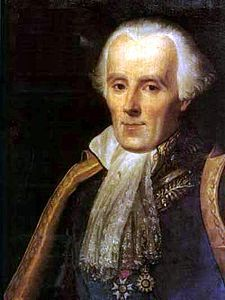
\includegraphics[height=2in,clip]{laplace}
  		\caption{Laplace}
	\end{center}
  	\end{figure}
  \end{column}
\end{columns}
\end{frame}


%%%%%%%%%%%%%%%%%%%%%%%%%%%%%%%%%%%%%%%%%%%%%%%%%%%%%%
%%%%%%%%%%%%%%%%%%%%%%%%%%%%%%%%%%%%%%%%%%%%%%%%%%%%%%
\begin{frame}{Evaluate $\pi$ by Random Sampling}

\begin{columns}
  \begin{column}{0.45\textwidth}
  	\begin{figure}
  	\begin{center}
  		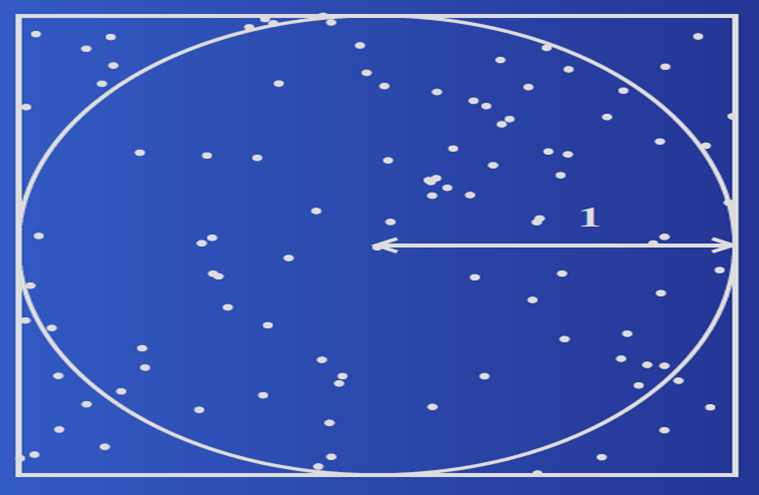
\includegraphics[height=2in,clip]{pi-circle}
	\end{center}
  	\end{figure}
  \end{column}
  \begin{column}{0.55\textwidth}
    \begin{itemize}
    \item Area of square, $A_s= 4$
    \item Area of circle, $A_c = \pi$
    \item Fraction of random points \\in circle
    \[p = \frac{A_c}{A_c} = \frac{\pi}{4}\]
    \item Random points = $N$
    \item Random points in circle  = $N_c$, $\therefore$
    \[p = \frac{N_c}{N}\:; \quad \pi = \frac{4N_c}{N}\]
    \end{itemize}
  \end{column}
\end{columns}
\end{frame}


%%%%%%%%%%%%%%%%%%%%%%%%%%%%%%%%%%%%%%%%%%%%%%%%%%%%%%
%%%%%%%%%%%%%%%%%%%%%%%%%%%%%%%%%%%%%%%%%%%%%%%%%%%%%%
\begin{frame}{Manhattan Project}

\begin{columns}
  \begin{column}{0.5\textwidth}
    \begin{itemize}
    \item The first human engineered nuclear detonation, 
    the Trinity Test in New Mexico.
    \item Active: 1942–1945
    \item Branch: U.S. Army Corps of Engineers
    \item Monte Carlo Pioneers:
    \begin{itemize}
      \item Enrico Fermi,
      \item Stanislaw Ulam,
      \item John von Neumann, 
      \item Robert Richtmeyer, 
      \item Nicholas Metropolis
    \end{itemize}
    \end{itemize}
  \end{column}
  \begin{column}{0.5\textwidth}
  	\begin{figure}
  	\begin{center}
  		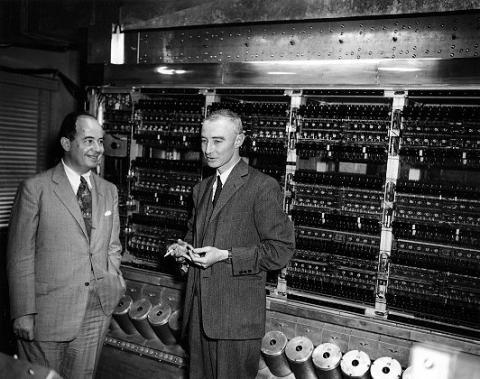
\includegraphics[height=1.75in,clip]{OppieNeumannMANIAC}
  		\caption{Oppenheimer, von Neumann, MANIAC}
  		%http://www.atomicheritage.org/history/computing-and-manhattan-project
	\end{center}
  	\end{figure}
  \end{column}
\end{columns}
\pause
Nicholas Metropolis, S.\ Ulam. ''The Monte Carlo Method," J\textit{ournal of the American Statistical Association}, \textbf{44}, No.\ 247. (Sep., 1949), 335-341.
\end{frame}


%%%%%%%%%%%%%%%%%%%%%%%%%%%%%%%%%%%%%%%%%%%%%%%%%%%%%%
%%%%%%%%%%%%%%%%%%%%%%%%%%%%%%%%%%%%%%%%%%%%%%%%%%%%%%
\begin{frame}{General Purpose MC Codes}

\begin{itemize}
\item \alert{MCNP}: developed at LANL, distributed via RSICC, \href{http://rsicc.ornl.gov}{http://rsicc.ornl.gov}
%
%\item PENELOPE: developed and maintained at U Barcelona, distributed via the Nuclear Energy Agency (http://www.nea.fr/abs/html/nea-1525.html

\item \alert{Geant4}: developed by a large collaboration in the HEP community, \href{ http://geant4.web.cern.ch/geant4/}{http://geant4.web.cern.ch/geant4/}

\item \alert{EGSnrc}: developed at NRC (Canada), \href{http://www.irs.inms.nrc.ca/EGSnrc/EGSnrc.html}{http://www.irs.inms.nrc.ca/EGSnrc/EGSnrc.html}

\item \alert{SERPENT}: Developed by Dr. Jaakko Leppanen, VTT, Finland, \href{ http://montecarlo.vtt.fi/}{http://montecarlo.vtt.fi/}

\item \alert{Shift}: developed at ORNL, distributed via RSICC, \href{http://rsicc.ornl.gov}{http://rsicc.ornl.gov}

\end{itemize}

\end{frame}


%%%%%%%%%%%%%%%%%%%%%%%%%%%%%%%%%%%%%%%%%%%%%%%%%%%%%%
%%%%%%%%%%%%%%%%%%%%%%%%%%%%%%%%%%%%%%%%%%%%%%%%%%%%%%
\begin{frame}{Evaluate $\pi$ by Random Sampling (math)}

\begin{columns}
  \begin{column}{0.3\textwidth}
  	\begin{figure}
  	\begin{center}
  		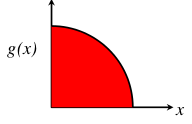
\includegraphics[height=0.75in,clip]{quarter-circle}
	\end{center}
  	\end{figure}
  \end{column}
  \begin{column}{0.7\textwidth}
    \begin{equation}
      g(x) = \sqrt{1 - x^2}	\qquad G = \int_0^1 g(x)dx = \frac{\pi}{4} \nonumber
    \end{equation}
  \end{column}
\end{columns}
\pause
\begin{equation}
  G = \int_0^1 g(x)dx = (1-0)\overline{g(x)} \nonumber
\end{equation}
Determine $\overline{g(x)}$ by random sampling:\\
\vspace*{0.5em}
\hspace*{2 em}for $k = 1, \dots, N$, chose $\hat{x}_k$ randomly on the interval $(0,1)$,
\[ \overline{g(x)} \equiv \frac{1}{N}\sum_{k=1}^N g(\hat{x}_k) = \frac{1}{N}\sqrt{1 - \hat{x}_k^2}\]

\end{frame}


%%%%%%%%%%%%%%%%%%%%%%%%%%%%%%%%%%%%%%%%%%%%%%%%%%%%%%
%%%%%%%%%%%%%%%%%%%%%%%%%%%%%%%%%%%%%%%%%%%%%%%%%%%%%%
\begin{frame}{Evaluate $\pi$ by Random Sampling (physics)}

\begin{columns}
  \begin{column}{0.3\textwidth}
  	\begin{figure}
  	\begin{center}
  		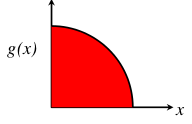
\includegraphics[height=0.75in,clip]{quarter-circle}
	\end{center}
  	\end{figure}
  \end{column}
  \begin{column}{0.7\textwidth}
    \begin{equation}
      g(x) = \sqrt{1 - x^2}	\qquad G = \int_0^1 g(x)dx = \frac{\pi}{4} \nonumber
    \end{equation}
  \end{column}
\end{columns}
\pause
\vspace*{0.5em}
G = area under curve, \\
\hspace*{0.75 em} = fraction of unit square under curve\\
\vspace*{0.5em}
\hspace*{2 em}for $k = 1, \dots, N$, chose $\hat{x}_k, \hat{y}_k$ randomly on the interval $(0,1)$,\\
\vspace*{0.5em}
$m_N$ = $\#$ of times in $N$ trials that $\hat{x}_k^2 + \hat{y}_k^2 \leq 1$,
\[G = \frac{m_N}{N}\]

\end{frame}



\end{document}
